\documentclass[compress, blue, hyperref={unicode, bookmarks=true, pdfpagemode=FullScreen}]{beamer}
\mode<presentation>
\usetheme{Madrid}
\useoutertheme[subsection=false]{smoothbars}
\beamertemplateshadingbackground{yellow!30}{white}
%\usepackage{tikz}
\usepackage[french]{babel}
\usepackage[utf8]{inputenc} 
\usepackage[T1]{fontenc} 
\usepackage{multicol}
\usepackage{color}
\usepackage{graphicx}
\usepackage[all]{xy}
\usepackage{array}
\setbeamertemplate{navigation symbols}{}


\usepackage{amsmath, amssymb, esint, amstext}
\setbeamertemplate{theorem begin}
{
\begin{\inserttheoremblockenv}
{Th\'eor\`eme}}

\setbeamerfont{frametitle}{size=\large}

\AtBeginSection[] {
  \begin{frame}[t]
    \frametitle{Plan}
      \tableofcontents[sectionstyle=show/shaded,subsectionstyle=hide]
  \end{frame}
} 

\title[SEME 2014]{Projet Axessim : Calcul de matrice d'imp\'edance pour la simulation num\'erique des lignes de transmission multi-conducteur}
\author[Projet Axessim ]{Propos\'e par T. Strub\\[1ex]
avec G. Doll\'e, N. Pham, A. Samake, A. Assmar, qui }
\institute[ ]{Semaine d'\'etude Maths-Entreprises
\vspace{.5cm}



\includegraphics[height=1cm]{Logos/unistra.jpg}
\hspace{3cm}

\includegraphics[height=1cm]{Logos/inr}
}
\date{Strasbourg, le 27 juin 2014}

%%%%%%%%%%%%%%                      Debut du document                             %%%%%%%%%%%%%%%


\begin{document}


%%%%%%%%%%%%%%                      Titre                             %%%%%%%%%%%%%%%
\begin{frame}
  \titlepage
\end{frame}





%%%%%%%%%%%%%%                      TOC                             %%%%%%%%%%%%%%%



\begin{frame}[allowframebreaks]
\frametitle{\Large Plan de la pr\'esentation }
\tableofcontents[hideallsubsections]
\end{frame}



%%%%%%%%%%%%%%                      Introduction                             %%%%%%%%%%%%%%%

\section[Intro.]{Introduction}\subsection{hack}
%------------------------------------------------------------------------------
\begin{frame}
  \frametitle{Probl\`eme physique}
  %JE VAIS
  Calculer les tensions $U(z,\omega) =(u_1 \cdots u_N)^T$ et les courants
  $I(z,\omega) = (I_1\cdots I_N)$ complexes dans un faisceau de conducteurs
  $w_i$, $i=1\cdots N$. Les cables sont entour\'es d'un blindage $w_0$. La forme
  du faisceau est fix\'ee dans le plan $(x,y)$ et invariante suivant $z$.
  \begin{center}
    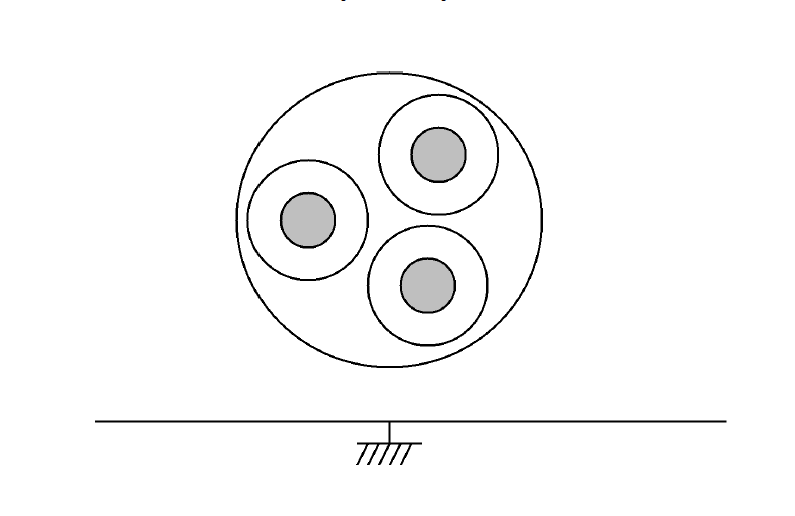
\includegraphics[height=4cm]{figures/f1}\\
    \small  Exemple de section d'un cable.
  \end{center}
\end{frame}
%------------------------------------------------------------------------------


\begin{frame}
\frametitle{Ligne de transmission}
\'Equation des lignes de transmissions ($j^2=-1$)
\begin{eqnarray*}
\frac{\partial U}{\partial z} =ZI, \quad Z=R+j\omega L,\\
\frac{\partial I}{\partial z} =YU, \quad Y=G+j\omega C.
\end{eqnarray*}
Matrices: 
Imp\'edance $Z$, R\'esistance $R$, Inductance $L$, Admittance $Y$, Conductance $G$, Capacit\'e
$C=L^{-1}.$\\[0.4cm]
Propri\'etes des matrices: 
\begin{itemize}
\item Sym\'etrique
\item D\'efinie positive
\end{itemize}

\end{frame} 

\begin{frame}
\frametitle{Probl\`eme}
Flux magn\'etique $\varphi(x,y)$. \\
Champ magn\'etique: d\'erive d'un potentiel vecteur 
$$B=\nabla \times (0,0,\varphi)^T.$$ et
$$\nabla\times B=(0,0,j_z)^T$$ avec
\begin{itemize}
\item  $j_z(x,y)$ : densit\'e de courant suivant $z$
\item  $I_i= \int _{w_i}j_z(x,y)dxdy$ :  courant
\end{itemize}
On a
\begin{equation}
-\Delta\varphi =
\begin{cases}
j_z \\ 
0 \qquad \text{sur } \Omega =w_0 \setminus \cup_i w_i,
\end{cases}
\end{equation} 
\end{frame}



%%%%%%%%%%%%%%                      modèle et assemblage matrice                            %%%%%%%%%%%%%%%


\section[Mtrice]{Probl\`eme}\subsection{prob1}
\begin{frame}
\frametitle{Sous forme de matrice}
%Consid\`ere le mod\`ele
%\begin{equation}
%-\Delta\varphi = j_z 
%\end{equation}
On peut \'ecrire
 \begin{equation}
 \tilde\varphi = \sum_k \phi_k \tilde{\varphi}_k
 \end{equation}
 avec $\tilde{\varphi}$ est solution de probl\`eme suivante 
 \begin{equation}
 \begin{cases}
 -\Delta{\varphi} = 0 \quad \text{sur } \Omega \\
 {\varphi} = \delta_{ij} 
 \end{cases}
 \end{equation}
 donc on a
 \begin{equation}
 \sum_j \phi_j \left( \int_{w_i}-\Delta\tilde{\varphi}_j \right) =I_i
 \end{equation}
 ou bien
 \begin{equation}
  \sum_j \phi_j \left( \int_{\partial w_i}-\nabla\tilde{\varphi}_j \right) \cdot n =I_i
 \end{equation}
 en d'\'eduit
  \begin{equation}
  \sum_j M_{ij}\phi_j =I_i \quad \forall i 
 \end{equation}
%
%\begin{eqnarray*}
%\frac{\partial U}{\partial z} =ZI, \quad Z=R+j\omega L,\\
%\frac{\partial I}{\partial z} =YU, \quad Y=G+j\omega C.
%\end{eqnarray*}


\end{frame} 

 \begin{frame}
\frametitle{Calcul la matrice M}
On a
\begin{equation}
  M_{ij} = \int_{\partial w_j} \frac{\partial\varphi_i}{\partial n}
\end{equation}
 Properties de la matrice $M$
 \begin{itemize}
 \item Sym\'etrique 
 \item D\'efinie positive
 \item Inversible
 \end{itemize}
 Ou bien
\begin{equation}
  M\phi =I \quad \text{ou bien } \phi =LI \quad \text{o\`u } L=M^{-1} 
\end{equation}


\end{frame} 

\begin{frame}
\frametitle{Calcul la matrice M}
Probl\`eme quand on a calculer directement l'int\'egrale : La matrice $M$ n'est plus sym\'etrique 
=> solution: formulation faiblement
\begin{equation}
\int_w -\Delta\varphi \psi =\int_w \nabla\varphi\nabla\psi - \int_{\partial w} \nabla\varphi\cdot n \psi =\int_{\partial w} \nabla\varphi\cdot n 
\end{equation}
avec $\psi \in H^1(w)$ satifait 
\begin{equation}
\psi(z) =
\begin{cases}
0 \qquad \text{ si } z\in w \\
1 \qquad \text{ si } z\in \partial w
\end{cases}
\end{equation} 


\end{frame} 


%%%%%%%%%%%%%%                      assemblage matrice                            %%%%%%%%%%%%%%%


\section[Cabs+blindages]{Cas des cables et des blindages}\subsection{prob2}
%------------------------------------------------------------------------------
\begin{frame}
  \frametitle{Cas des cables et des blindages}
  \begin{columns}[T]
    \column{0.5\linewidth}
    \begin{itemize}
      \item Blindage de r\'ef\'erence $w_0$ et $N$ conducteurs $w_1 \cdots w_N$
      \item Chaque conducteur $w_i$ contient $N^i_{int}$ sous conducteurs
      \item Chaque conducteur $w_i$ matrice d'inductance $L_{int}^i$
      \item $L_{ext}$ : matrice d'inductance des conducteurs ext\'erieurs
    \end{itemize}
    \column{0.5\linewidth}
    \begin{center}
      \begin{tikzpicture}[scale=0.6]
        \draw [thick,fill=cyan!10!white]  (0,0) node (v1) {} ellipse (4 and 4);
        \node at (-4.5,0) {$w_0$};
        \draw [thick,fill=cyan] (-2,0) ellipse (1 and 1);
        \draw [thick,fill=cyan!40!white] (2,0) ellipse (1.5 and 1.5);
        \node at (-2,1.7) {$w_1$};
        \node at (2,1.7) {$w_2$};

        %      \draw [thick,fill=cyan] (2,0) ellipse (0.5 and 0.5);
        \draw [thick,fill=cyan] (2,0.6) ellipse (0.5 and 0.5);
        \draw [thick,fill=cyan] (2,-0.6) ellipse (0.5 and 0.5);
      \end{tikzpicture}
    \end{center}
  \end{columns}
\end{frame}
%------------------------------------------------------------------------------


%------------------------------------------------------------------------------
\begin{frame}
\frametitle{Cas des cables et des blindages}
On obtient
\[ \left[ \begin{array} {c}
\phi_{ext} \\
\tilde{\phi}^1_{int}  \\
\vdots \\
\tilde{\phi}^{N_{int}}_{int} \end{array}  \right]  =
\left[ \begin{array} {cccc}
L_{ext} & & & \\
  & L^1_{int}& &  \\
 & &\ddots &  \\
 & & & L^{N_{int}}_{int} \end{array}  \right]
 \left[ \begin{array} {c}
\tilde{I}_{ext} \\
I^1_{int}  \\
\vdots \\
I^{N_{int}}_{int} \end{array}  \right]
\] \\[0.6cm]
on en d\'eduit
\[ \left[ \begin{array} {c}
\phi_{ext} \\
\tilde{\phi}_{int} \end{array}  \right]  =
\left[ \begin{array} {cc}
L_{ext} & \\
  & L_{int}  \end{array}  \right]
 \left[ \begin{array} {c}
\tilde{I}_{ext} \\
I_{int} \end{array}  \right]
\] \\[0.6cm]
($\tilde{\phi}_{int}$ potentiel int\'erieux calcul\'e avec une r\'ef\'erence sur les blindages)
\end{frame}
%------------------------------------------------------------------------------


%------------------------------------------------------------------------------
\begin{frame}
\frametitle{Cas des cables et des blindages}
Changement de variables
\begin{equation}
\phi_{int} = \tilde{\phi}_{int} +\delta^T \phi_{ext},
\end{equation}
avec $\delta$ : matrice de taille $N_{ext}\times N_{int}$ et
\begin{equation}
\delta(i,j)=
\begin{cases}
1 \qquad \text{si le conducteur $j+N_{ext}$ est dans le conducteur $i$,} \\
0 \qquad \text{sinon.}
\end{cases}
\end{equation}
De plus,
\begin{equation}
\phi_{ext} = L\tilde{I}_{ext}=L(I_{ext}-\delta I_{int})
\end{equation}
La matrice d'inductance globale
\[ \left[ \begin{array} {c}
\phi_{ext} \\
\phi_{int} \end{array}  \right]  =
L
 \left[ \begin{array} {c}
I_{ext} \\
I_{int} \end{array}  \right]
\]
avec
\[ L = P_I^T \left[ \begin{array} {cc}
L_{ext} &0 \\
0 & L_{int} \end{array}  \right] P_I , \qquad
P_I
\left[ \begin{array} {cc}
1 & -\delta \\
0 & 1 \end{array}  \right]
 \]

\end{frame}
%------------------------------------------------------------------------------


%%%%%%%%%%%%%%                      Discussions et perspectives                              %%%%%%%%%%%%%%%

\section{Conclusions et perspectives}\subsection{hack}
\begin{frame}
Bilan :
\begin{itemize}
\item AAA
\item BBB
\item CCC
\end{itemize}
\vspace{1cm}
\pause
Perspectives :
\begin{itemize}
\item Cas g\'en\'eral
\item Probl\`eme global -> local
\item Autres 
\item Modèles plus complexes
\end{itemize}
\end{frame}


\begin{frame}
\begin{center}
\Huge Merci de votre attention !
\end{center}
\end{frame}


%%%%%%%%%%%%%%                  References et FIN                                   %%%%%%%%%%%%%%%
\tiny
\include{ref}





\end{document} 



